\documentclass{article}
\usepackage[utf8]{inputenc}
\usepackage{float}
\usepackage{graphicx}

\title{DB PRAKTIKUM APEX}
\author{Ahmad Agung Tawakkal\\1184015\\D4 TI 2B}
\date{November 2019}

\graphicspath{{Images/}}

\begin{document}

\maketitle

\newpage

\section{Tutorial Apex}
    \subsection{Apa yang dimaksud dengan Oracle Application Express (APEX)?}
    \paragraph{}Oracle Application Express (APEX) adalah platform pengembangan \textit{low-code} yang memungkinkan Anda membangun aplikasi perusahaan yang dapat diskalakan dan aman, dengan fitur kelas dunia, yang dapat digunakan di mana saja.
    \subsection{Pembuatan Akun}
    \paragraph{}Untuk membuat akun anda dapat mengikuti langkah-langkah berikut;
        \begin{itemize}
            \item Buka link https://apex.oracle.com/en/
                \begin{figure}[ht]
                    \centerline{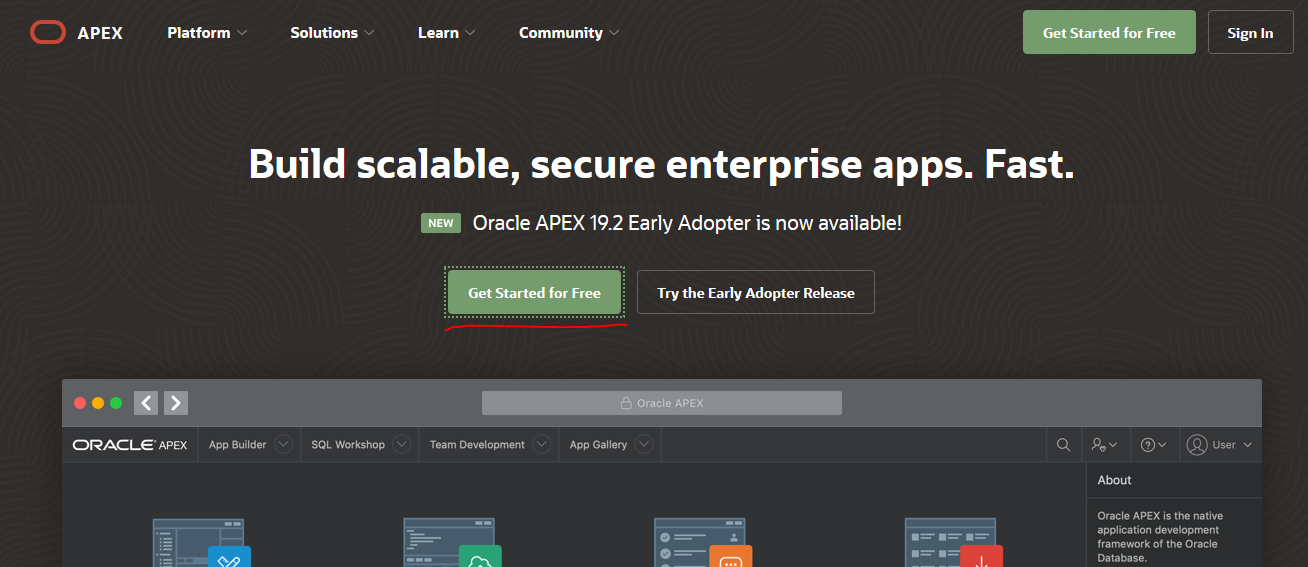
\includegraphics[width=7cm]{Capture.PNG}}
                    \caption{Gambar 1.0}
                \end{figure}
            \item Kemudian klik tombol \textit{Get Started for Free}
            \item Pilih \textit{Request a Free Workspace} 
                 \begin{figure}[ht]
                    \centerline{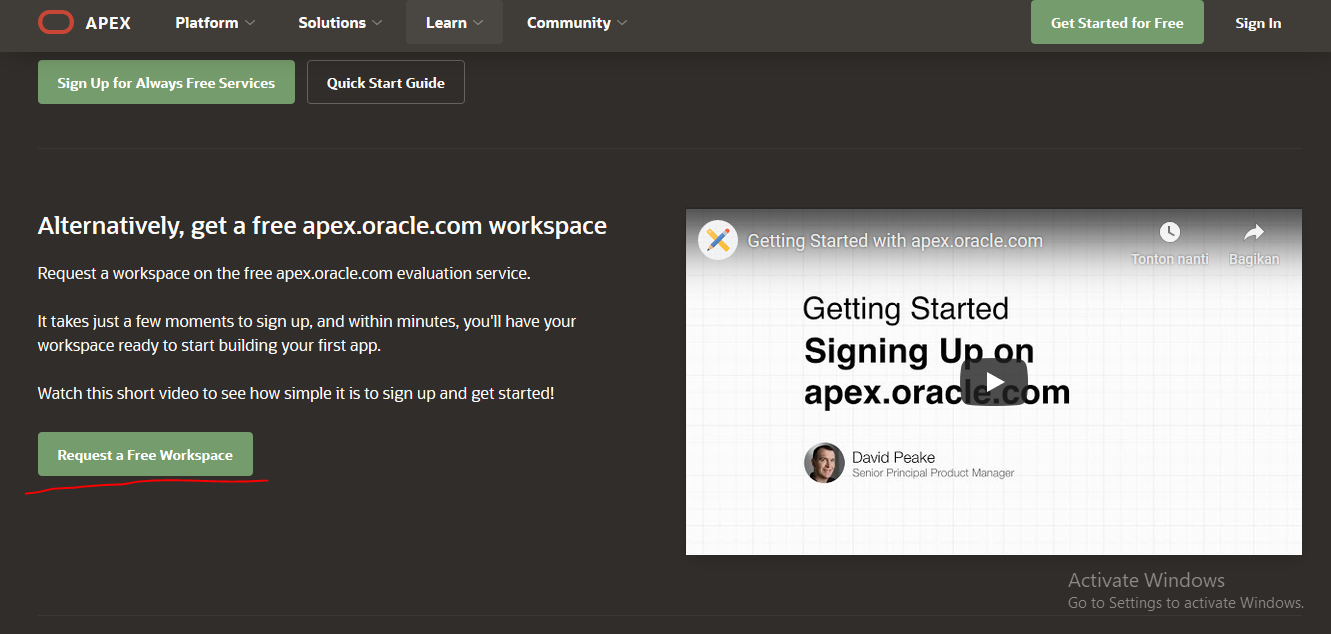
\includegraphics[width=7cm]{Capture1.PNG}}
                    \caption{Gambar 1.1}
                \end{figure}
            
            \newpage
            \item Isi untuk memenuhi persyaratan
                \begin{figure}[ht]
                    \centerline{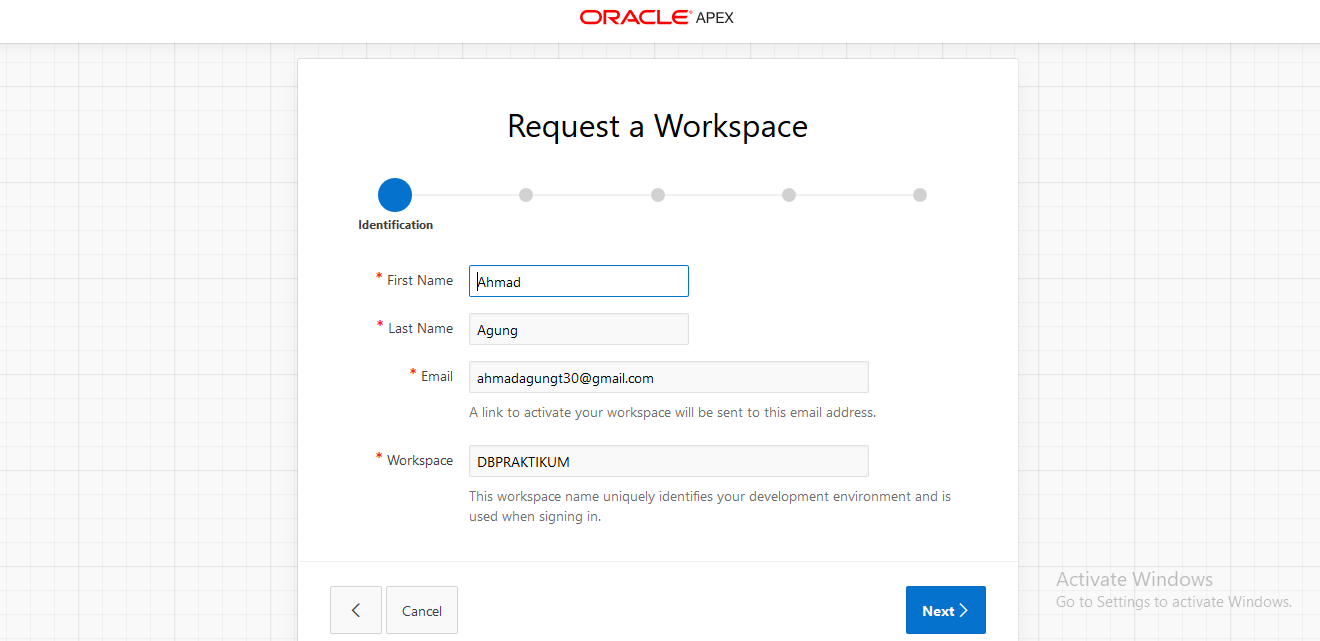
\includegraphics[width=5cm]{Capture2.PNG}}
                    \caption{Gambar 1.2}
                \end{figure}
                \begin{figure}[ht]
                    \centerline{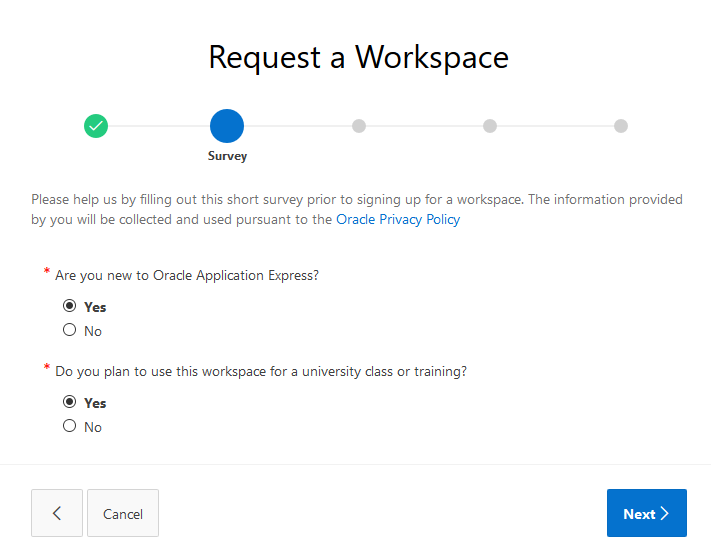
\includegraphics[width=5cm]{Capture3.PNG}}
                    \caption{Gambar 1.3}
                \end{figure}
                \begin{figure}[ht]
                    \centerline{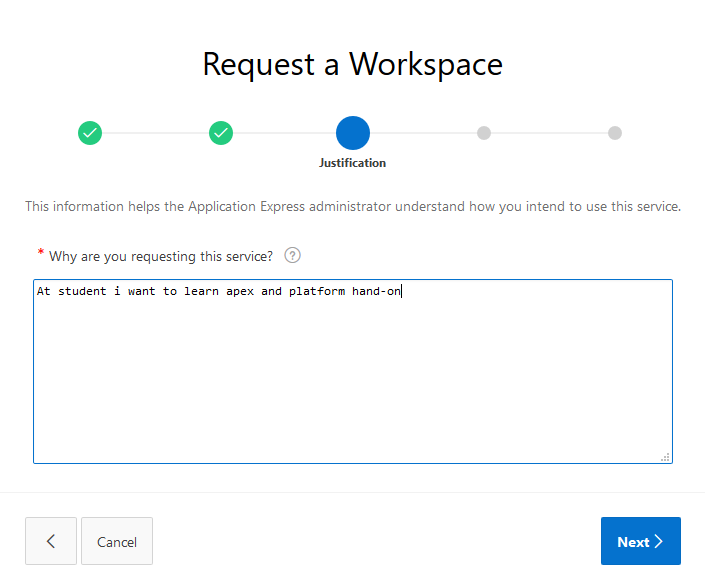
\includegraphics[width=5cm]{Capture4.PNG}}
                    \caption{Gambar 1.4}
                \end{figure}
                \begin{figure}[ht]
                    \centerline{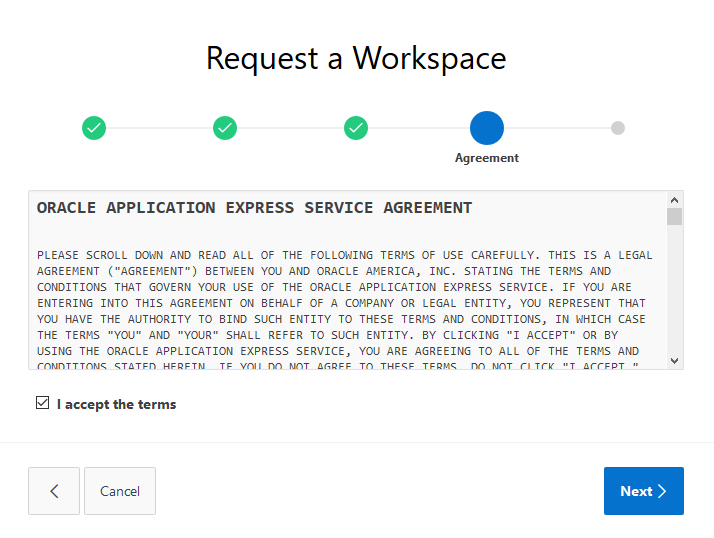
\includegraphics[width=5cm]{Capture5.PNG}}
                    \caption{Gambar 1.5}
                \end{figure}
                \begin{figure}[ht]
                    \centerline{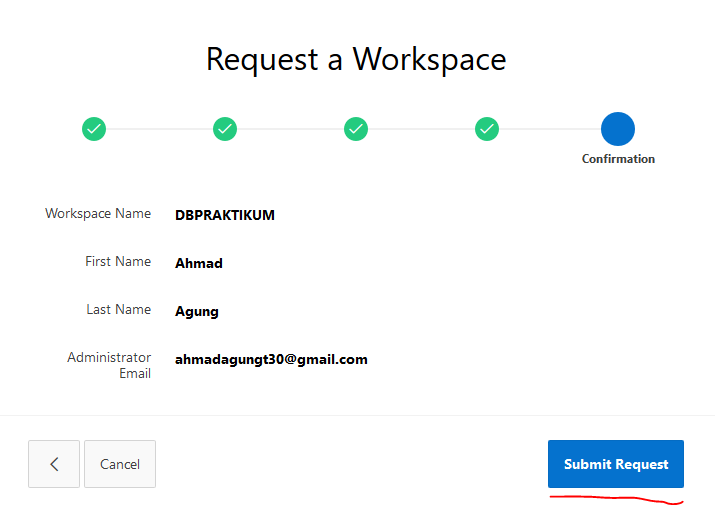
\includegraphics[width=5cm]{Capture6.PNG}}
                    \caption{Gambar 1.6}
                \end{figure}
        \end{itemize}
        
    \newpage
    \subsection{Membuat App Pada APEX}
        \begin{itemize}
            \item Masuk ke menu \textit{login} APEX 
                \begin{figure}[ht]
                    \centerline{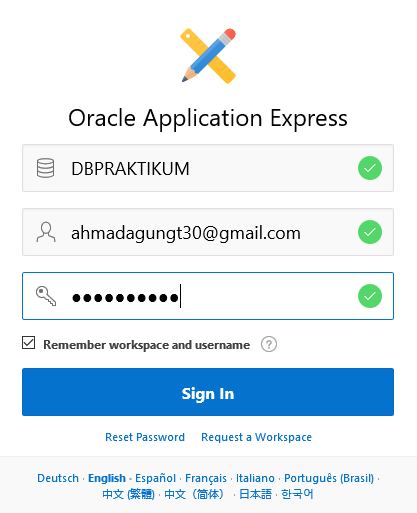
\includegraphics[width=3cm]{Capture7.PNG}}
                    \caption{Gambar 2.0}
                \end{figure}
            \newpage
            \item Pilih \textit{App Builder}
                \begin{figure}[ht]
                    \centerline{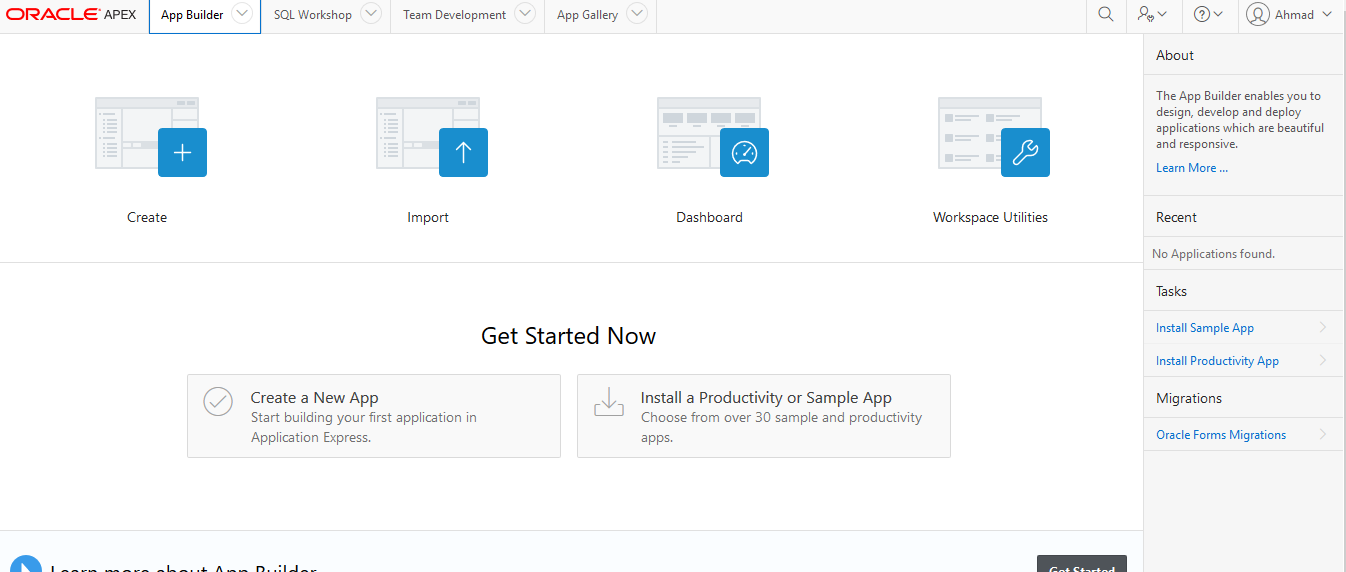
\includegraphics[width=5cm]{Capture8.PNG}}
                    \caption{Gambar 2.1}
                \end{figure}
            \item Kemudian pilih \textit{Create a New App} 
                \begin{figure}[ht]
                    \centerline{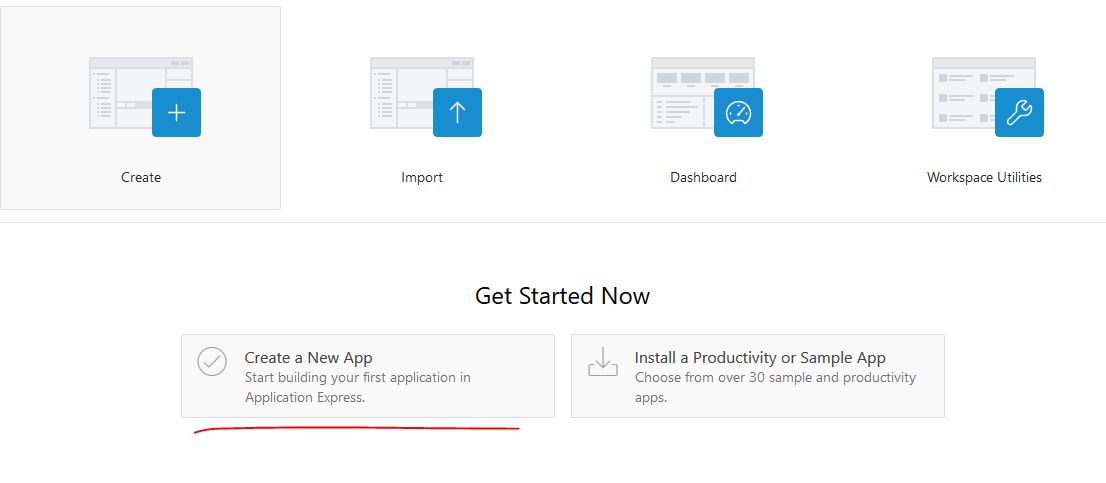
\includegraphics[width=5cm]{Capture9.PNG}}
                    \caption{Gambar 2.2}
                \end{figure}
            \item Pastikan anda memiliki data berbentuk CSV, pilih \textit{From a File} 
                \begin{figure}[ht]
                    \centerline{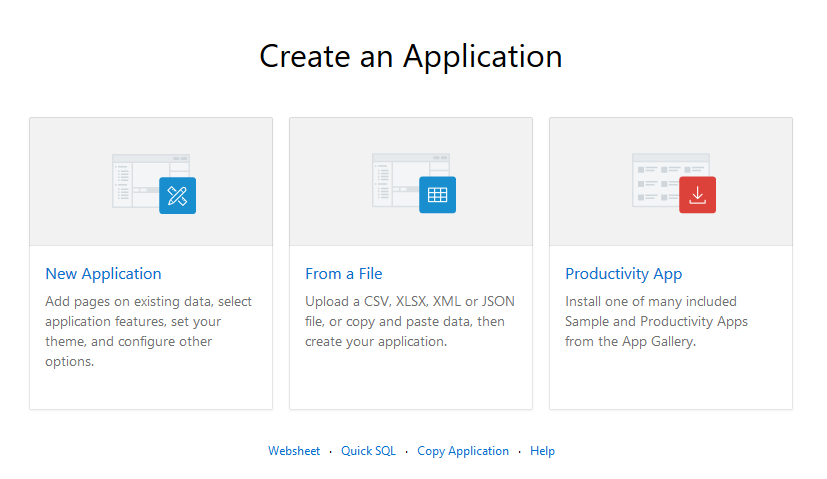
\includegraphics[width=5cm]{Capture10.PNG}}
                    \caption{Gambar 2.3}
                \end{figure}
            \newpage
            \item Pilih file CSV
                \begin{figure}[ht]
                    \centerline{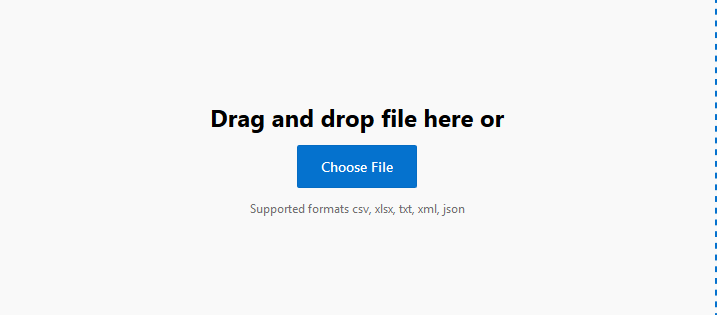
\includegraphics[width=5cm]{Capture11.PNG}}
                    \caption{Gambar 2.4}
                \end{figure}
                \begin{figure}[ht]
                    \centerline{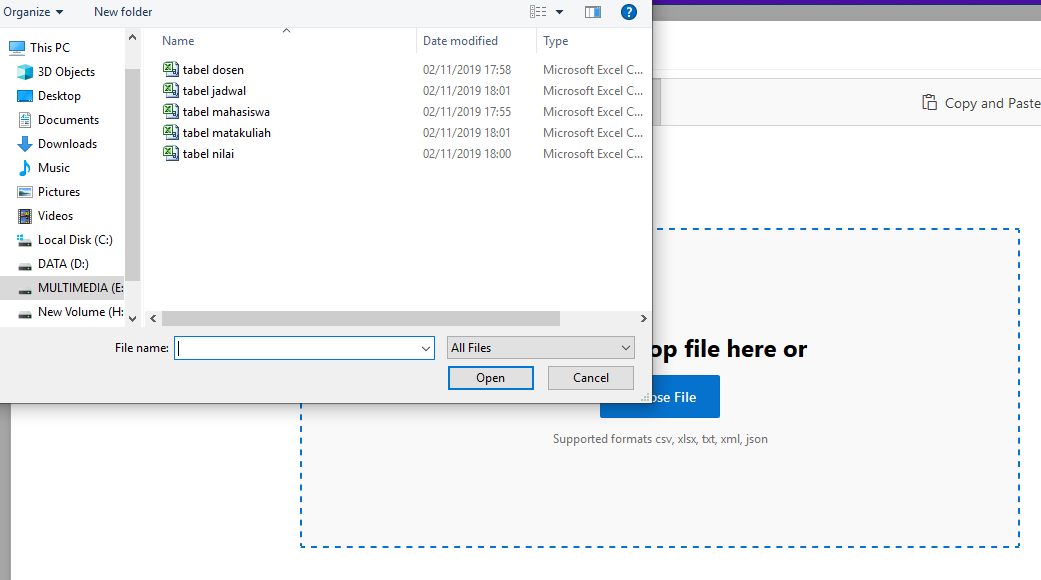
\includegraphics[width=5cm]{Capture12.PNG}}
                    \caption{Gambar 2.5}
                \end{figure}
            \item Tambahkan nama tablenya, kemudian \textit{load data}
                \begin{figure}[ht]
                    \centerline{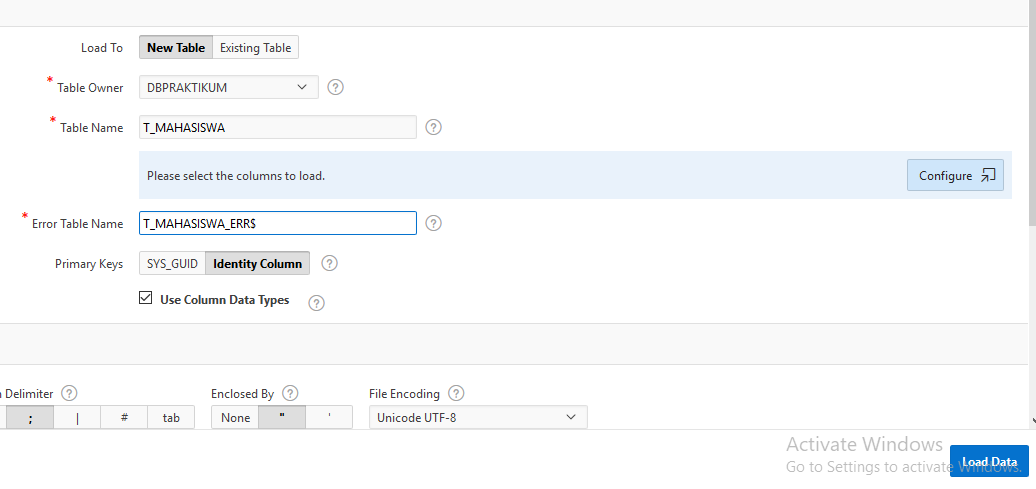
\includegraphics[width=5cm]{Capture13.PNG}}
                    \caption{Gambar 2.6}
                \end{figure}
            \newpage
            \item Jika selesai load data, jangan lansung diabuat aplikasinya karena kita akan menambahkan tabel lagi. Klik tanda silang pada ujung kanan atas.
                \begin{figure}[ht]
                    \centerline{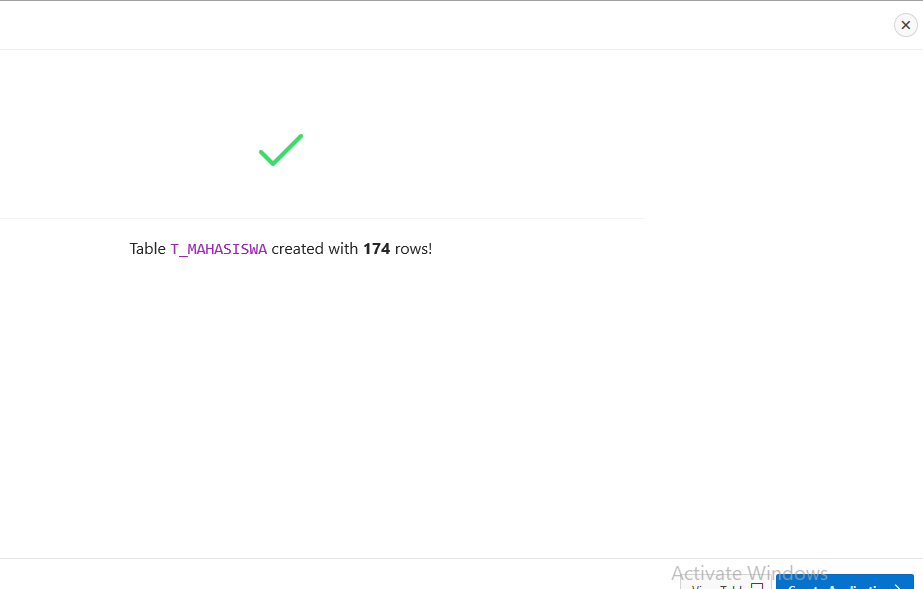
\includegraphics[width=5cm]{Capture14.PNG}}
                    \caption{Gambar 2.7}
                \end{figure}
            \item Kemudian masuk ke \textit{SQL Command}
                \begin{figure}[ht]
                    \centerline{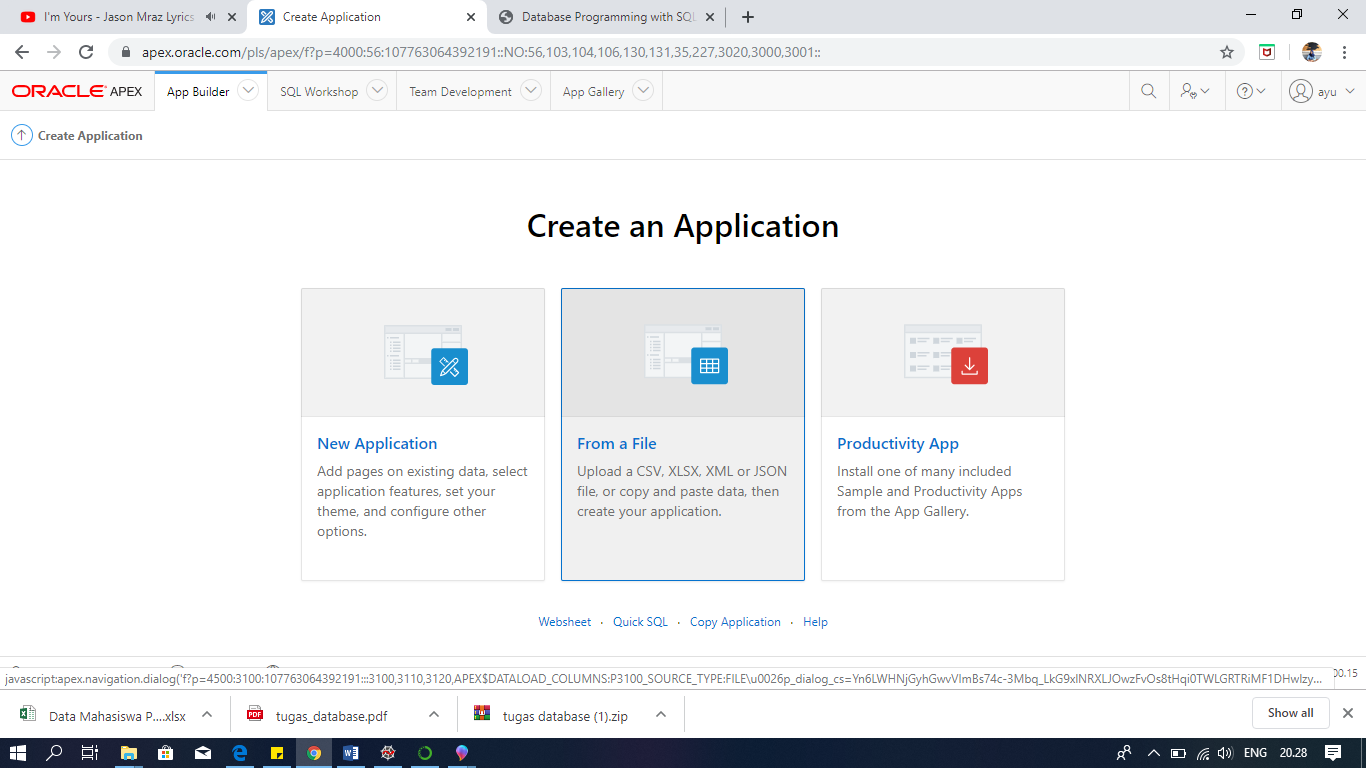
\includegraphics[width=5cm]{Untitled.PNG}}
                    \caption{Gambar 2.8}
                \end{figure}
            \newpage
            \item Kita akan menghapus \textit{id} dari setiap tabelnya dengan menambahkan \textit{scrypt} seperti pada gambar dibawah ini. Namun kita harus \textit{ran} satu persatu di setiap tabel columny id yang akan dihapus, dan tidak bisa lansung sekaligus. Contohnya : alter tabel t\_mahasiswa drop column id;
                \begin{figure}[ht]
                    \centerline{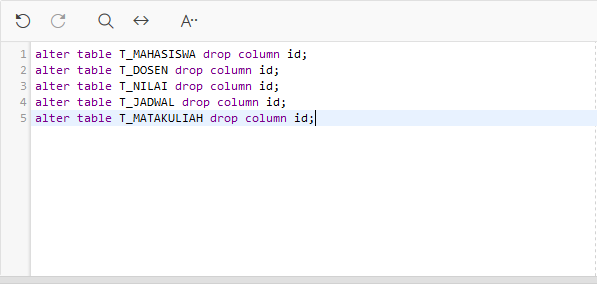
\includegraphics[width=10cm]{baru.PNG}}
                    \caption{Gambar 2.9}
                \end{figure}
            \item Setelah dihapus selanjutnya kita menambahkan \textit{primary key} pada tebel mahasiswa, dosen, dan matakuliah.
                \begin{figure}[ht]
                    \centerline{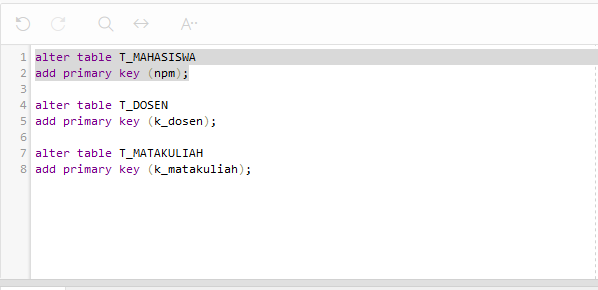
\includegraphics[width=10cm]{baru1.PNG}}
                    \caption{Gambar 2.10}
                \end{figure}
                \newpage
                \begin{figure}[ht]
                    \centerline{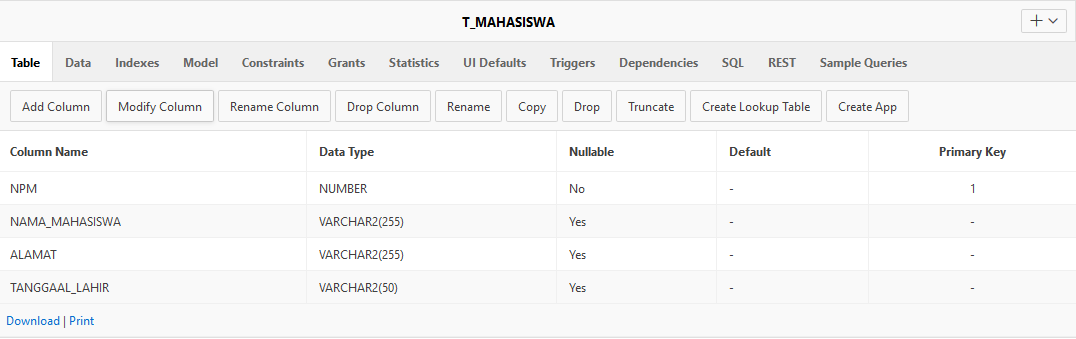
\includegraphics[width=9cm]{mahasiswa.PNG}}
                    \caption{Gambar 2.11 NPM jadi \textit{Primary Key} pada tabel Mahasiswa}
                \end{figure}
                \begin{figure}[ht]
                    \centerline{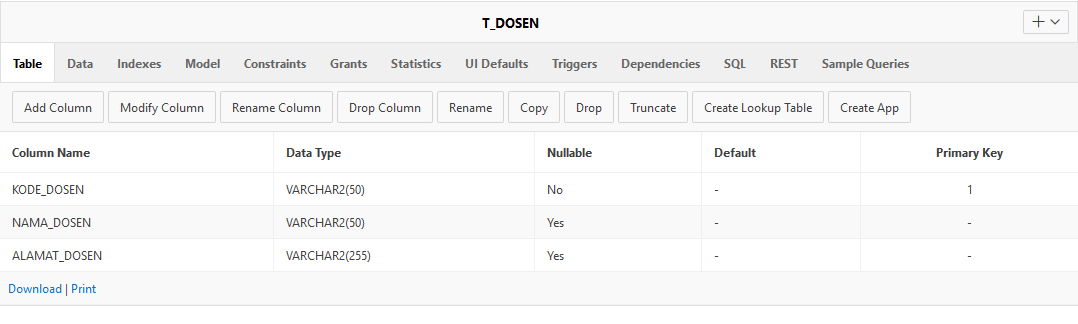
\includegraphics[width=9cm]{dosen.PNG}}
                    \caption{Gambar 2.12 Kode Dosen jadi \textit{Primary Key} pada tabel Dosen}
                \end{figure}
                \begin{figure}[ht]
                    \centerline{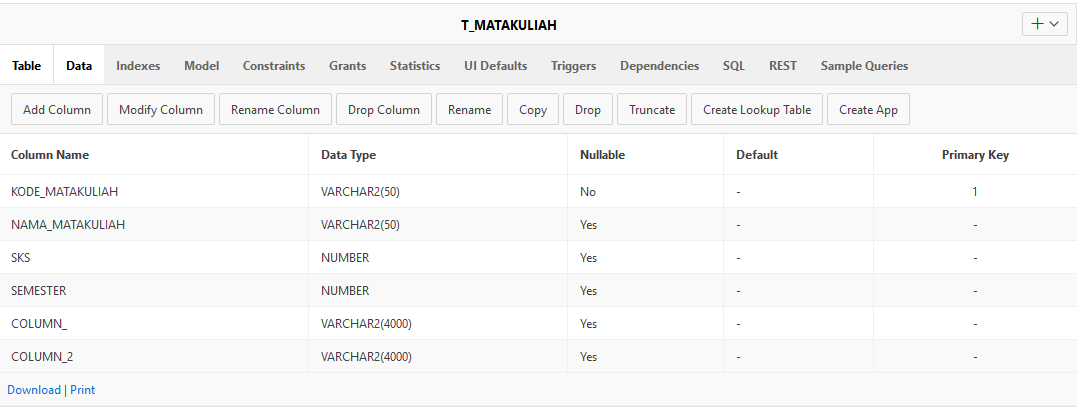
\includegraphics[width=9cm]{matkul.PNG}}
                    \caption{Gambar 2.13 Kode matakuliah jadi \textit{Primary Key} pada tabel Matakuliah}
                \end{figure}
            \newpage
            \item Kemudian jika telah selesai menambahkan table mahasiswa, dosen, matakuliah, jadwal, dan nilai selanjutnya membuat aplikasinya.
                \begin{figure}[ht]
                    \centerline{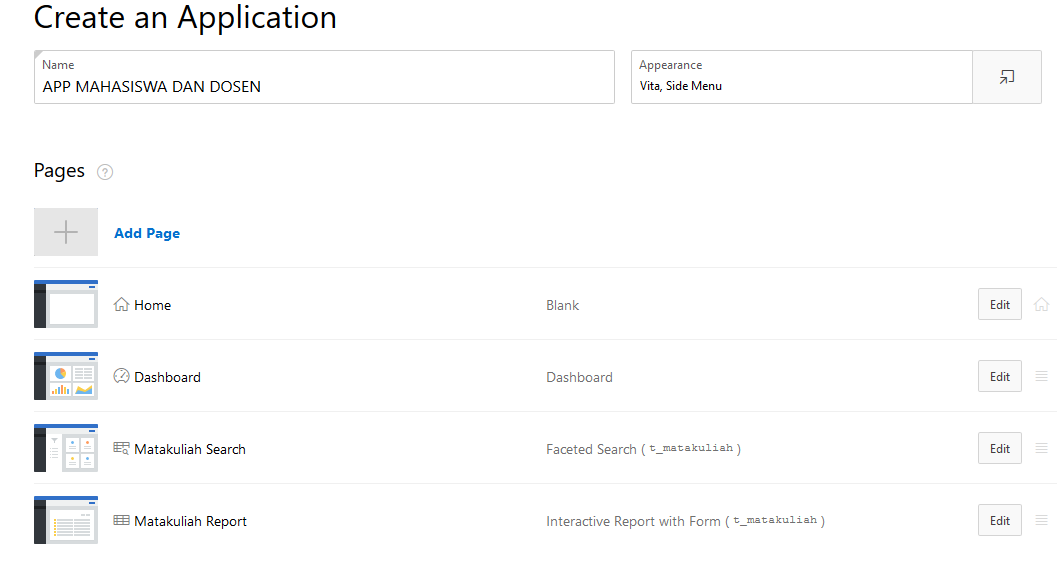
\includegraphics[width=5cm]{Capture15.PNG}}
                    \caption{Gambar 2.14}
                \end{figure}
            \item Pilih \textit{Interactive Report}
                \begin{figure}[ht]
                    \centerline{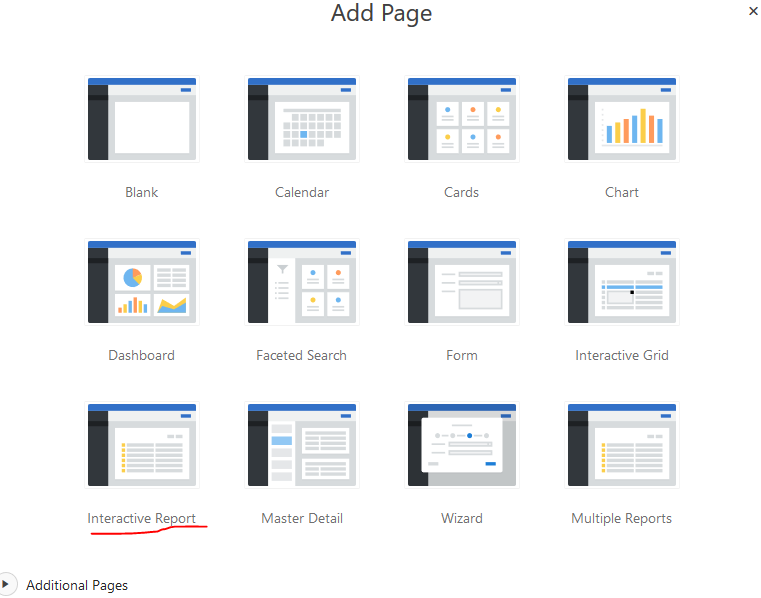
\includegraphics[width=5cm]{Capture16.PNG}}
                    \caption{Gambar 2.15}
                \end{figure}
            \newpage
            \item Tambahkan nama \textit{report}, dan memilih tabel. Jika anda ingin membuat tabel lebih bagus anda dapat menambahkan icon pada table.
                \begin{figure}[ht]
                    \centerline{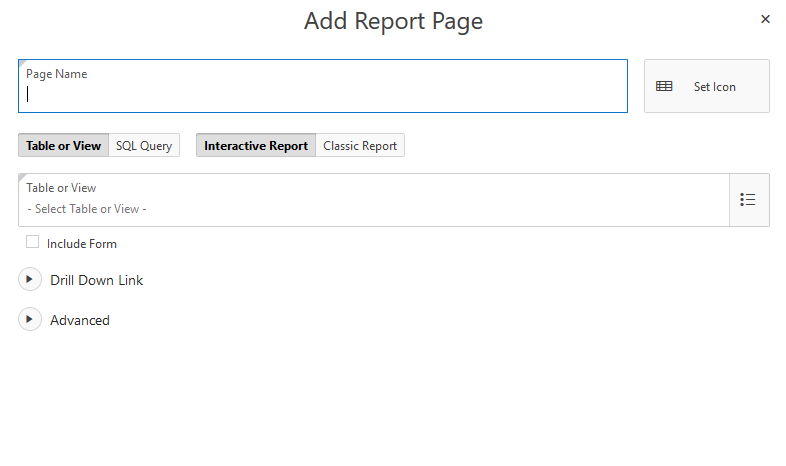
\includegraphics[width=5cm]{Capture17.PNG}}
                    \caption{Gambar 2.16}
                \end{figure}
                \begin{figure}[ht]
                    \centerline{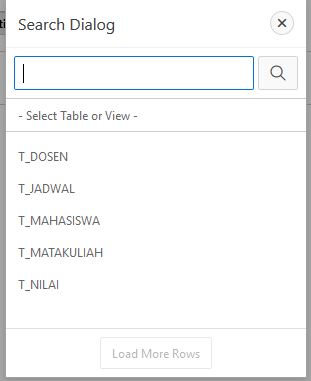
\includegraphics[width=3cm]{Capture19.PNG}}
                    \caption{Gambar 2.17}
                \end{figure}
                \begin{figure}[ht]
                    \centerline{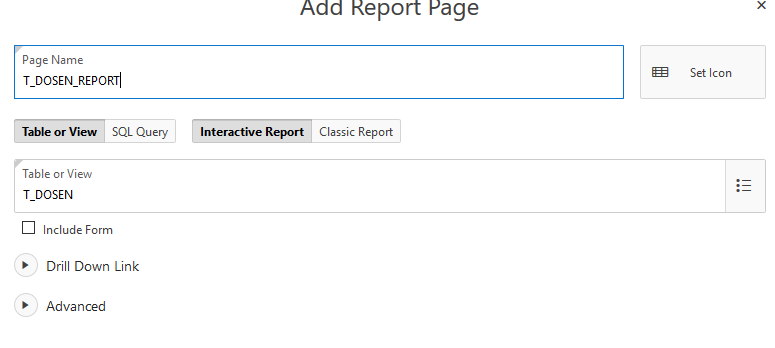
\includegraphics[width=5cm]{Capture18.PNG}}
                    \caption{Gambar 2.18}
                \end{figure}
            \newpage
            
            \item Setelah menambahkan tabel mahasiswa, dosen, dan matakuliah, selanjtunya anda membuat \textit{report} dengan menambahkan \textit{SQL Query}.Contohnya, menampilkan nama dosen dari kode dosen dengan memakai \textit{inner join} 
                \begin{figure}[ht]
                    \centerline{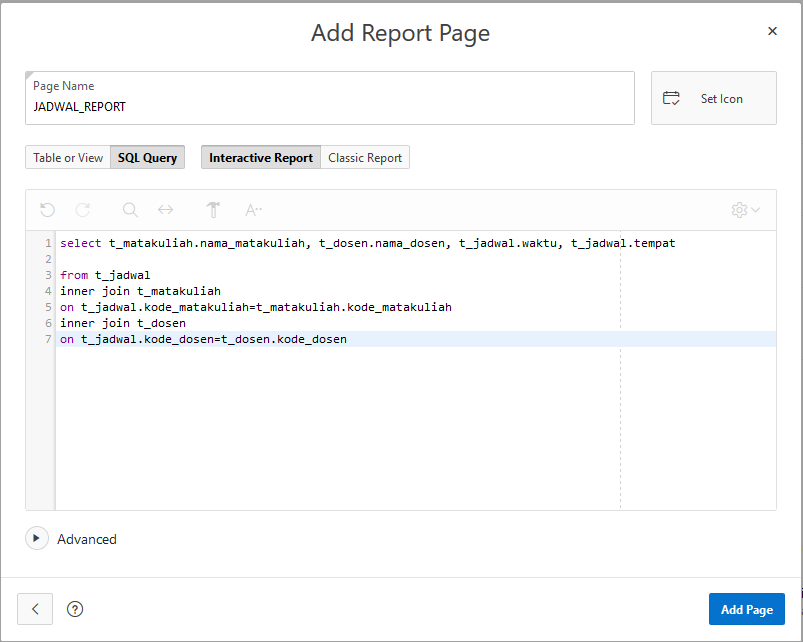
\includegraphics[width=7cm]{reportjadwal.PNG}}
                    \caption{Gambar 2.19}
                \end{figure}
                \begin{figure}[ht]
                    \centerline{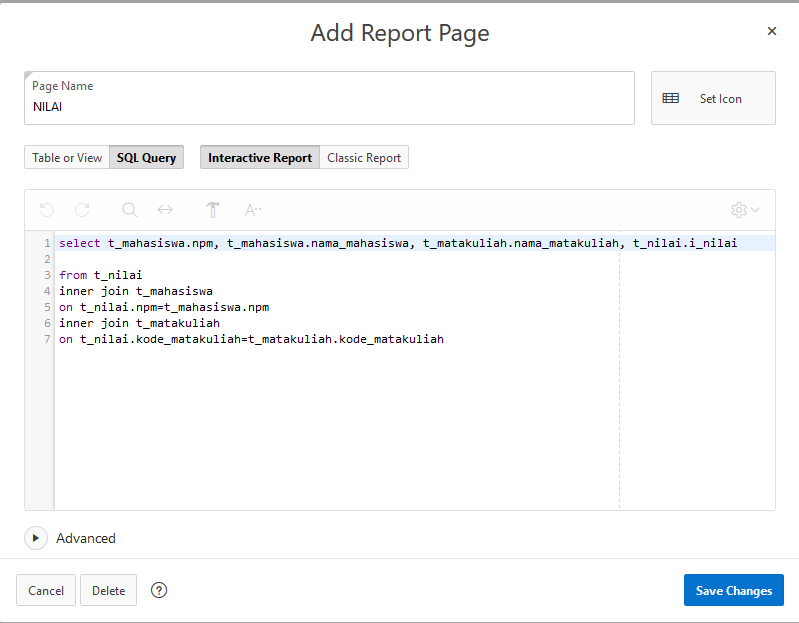
\includegraphics[width=7cm]{reportnilai.PNG}}
                    \caption{Gambar 2.21}
                \end{figure}
            \item Selanjutnya anda tinggal membuat aplikasinya dengan menekan \textit{create application}
                \begin{figure}[ht]
                    \centerline{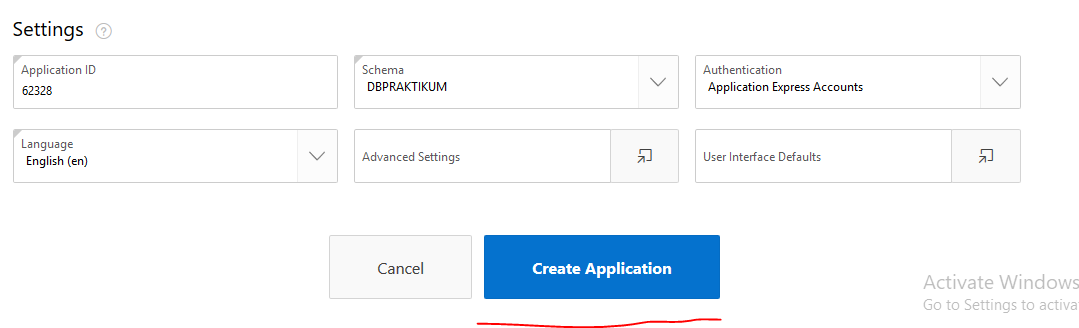
\includegraphics[width=5cm]{Capture21.PNG}}
                    \caption{Gambar 2.20}
                \end{figure}
            \item Tunggu hingga selesai pembuatan aplikasinya
                \begin{figure}[ht]
                    \centerline{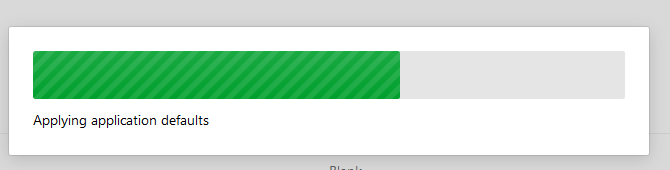
\includegraphics[width=5cm]{Capture22.PNG}}
                    \caption{Gambar 2.21}
                \end{figure}
            \newpage
            \item Pilih \textit{Run Application} 
                \begin{figure}[ht]
                    \centerline{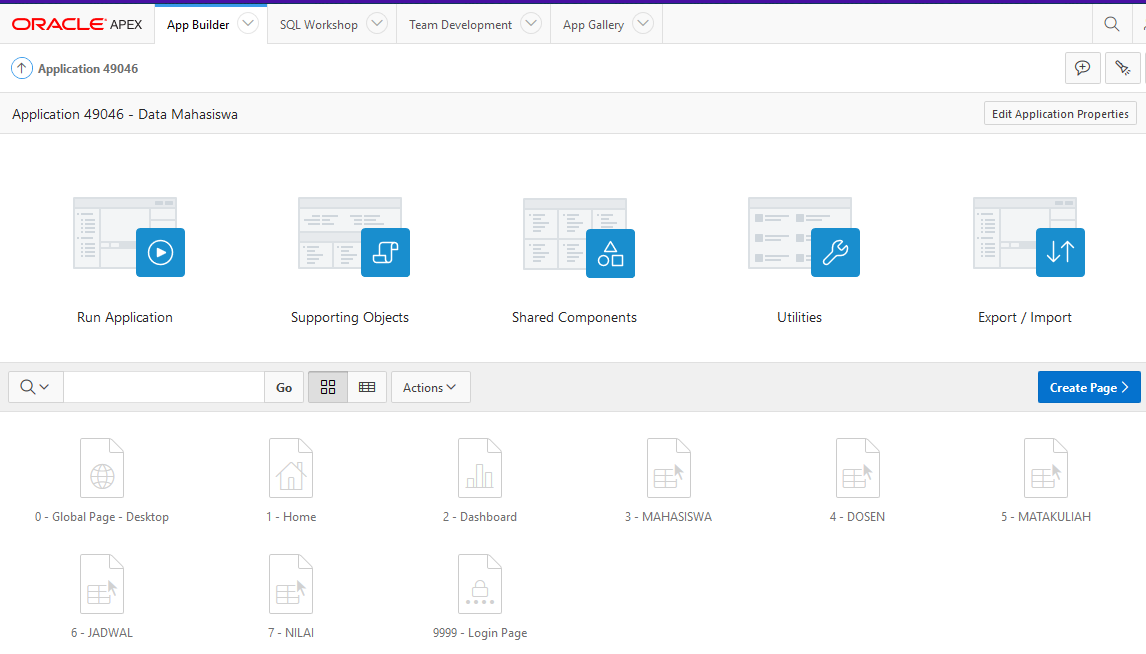
\includegraphics[width=5cm]{RUN.PNG}}
                    \caption{Gambar 2.22}
                \end{figure}
            \item Masukan \textit{email} dan \textit{password}
                \begin{figure}[ht]
                    \centerline{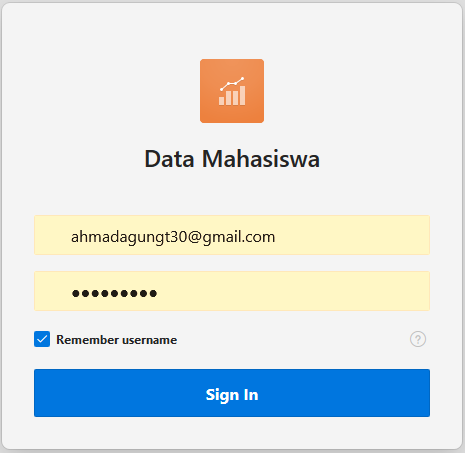
\includegraphics[width=5cm]{masuk.PNG}}
                    \caption{Gambar 2.23}
                \end{figure}
            \item Aplikasinya telah jadi dan siap untuk digunakan
                \begin{figure}[ht]
                    \centerline{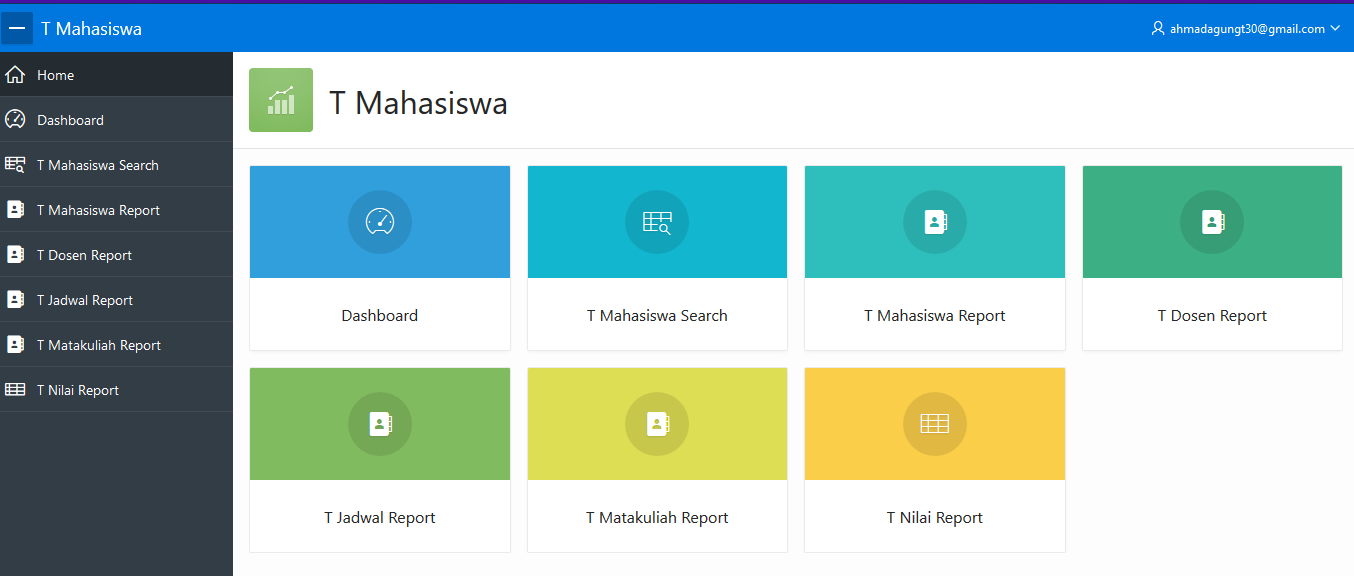
\includegraphics[width=8cm]{Capture25.PNG}}
                    \caption{Gambar 2.24}
                \end{figure}
        \end{itemize}
    \newpage
    \subsection{Akun}
        \begin{itemize}
            \item \textit{Link} : https://apex.oracle.com/pls/apex/f?p=49046:LOGIN\_DESKTOP:15349806496009:::::
            \item \textit{User} : ahmadagungt30@gmail.com
            \item \textit{Pass} : Ahmad3010
        \end{itemize}
        
        
\end{document}
